\documentclass{standalone}
\usepackage{pgfplots}
\pgfplotsset{compat=1.18}
\usepackage{xcolor}
\usetikzlibrary{calc,patterns,pgfplots.statistics} % Removed pgfplots.3d

% Define colors from Style Guide
\definecolor{Garnet}{HTML}{73000A}
\definecolor{Gray70}{gray}{0.70}

% Global PGFPlots settings per Style Guide
\pgfplotsset{
    every axis/.style={
        axis line style={draw=black, line width=0.6pt},
        tick style={draw=black, line width=0.6pt},
        tick label style={font=\footnotesize\color{black}},
        label style={font=\small\color{black}},
        grid=both,
        grid style={draw=Gray70, line width=0.4pt},
        legend style={
            draw=none,
            font=\footnotesize\color{black},
            fill=white,
        },
        title style={font=\small\color{black}}, % No titles used usually
        ybar,
        bar width=12pt, % Adjusted for visibility
        ymin=0,
    },
    barstyle/.style={
        draw=black,
        fill=Garnet,
        fill opacity=0.6,
        line width=0.6pt
    }
}

\begin{document}
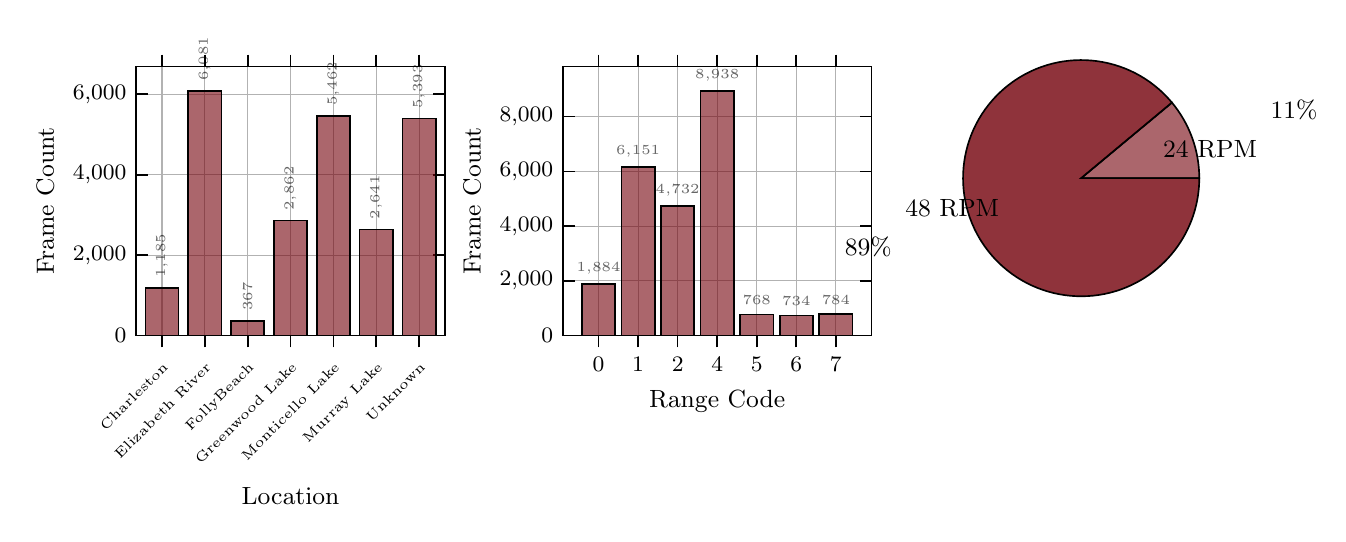
\begin{tikzpicture}
    % Chart 1: Frames by Location
    \begin{axis}[
        name=plot1,
        width=5.5cm, height=5cm,
        symbolic x coords={Charleston, Elizabeth River, FollyBeach, Greenwood Lake, Monticello Lake, Murray Lake, Unknown},
        xtick=data,
        xticklabel style={rotate=45, anchor=north east, font=\tiny},
        ylabel={Frame Count},
        xlabel={Location},
        enlarge x limits=0.1,
        nodes near coords,
        nodes near coords style={font=\tiny\color{black}, rotate=90, anchor=west}
    ]
        \addplot[barstyle] coordinates {
            (Charleston,1185)
            (Elizabeth River,6081)
            (FollyBeach,367)
            (Greenwood Lake,2862)
            (Monticello Lake,5462)
            (Murray Lake,2641)
            (Unknown,5393)
        };
    \end{axis}

    % Chart 2: Frames by Range Code
    \begin{axis}[
        name=plot2,
        at={(plot1.south east)},
        anchor=south west,
        xshift=1.5cm,
        width=5.5cm, height=5cm,
        symbolic x coords={0,1,2,4,5,6,7},
        xtick=data,
        ylabel={Frame Count},
        xlabel={Range Code},
        enlarge x limits=0.15,
        nodes near coords,
        nodes near coords style={font=\tiny\color{black}}
    ]
        \addplot[barstyle] coordinates {
            (0,1884)
            (1,6151)
            (2,4732)
            (4,8938)
            (5,768)
            (6,734)
            (7,784)
        };
    \end{axis}

    % Chart 3: Frames by Speed (RPM) - PIE CHART
    \begin{scope}[shift={(12cm,2cm)}]
        \pgfmathsetmacro{\radius}{1.5}
        \pgfmathsetmacro{\angle}{39.79}  % (2651/23991)*360 ≈ 39.79°

        % Slice 1: 24 RPM (0° to ~39.79°)
        \path[fill=Garnet, fill opacity=0.6, draw=black, line width=0.6pt]
            (0,0) -- (0:\radius cm) arc (0:\angle:\radius cm) -- cycle;

        % Slice 2: 48 RPM (~39.79° to 360°)
        \path[fill=Garnet, fill opacity=0.8, draw=black, line width=0.6pt]
            (0,0) -- (\angle:\radius cm) arc (\angle:360:\radius cm) -- cycle;

        % Labels with percentages - positioned outside pie
        \node[font=\small\color{black}, inner sep=0pt, anchor=west] at (19.9:1.1cm) {24 RPM};
        \node[font=\small\color{black}, inner sep=0pt, anchor=east] at (199.9:1.1cm) {48 RPM};

        % Percentage values
        \node[font=\small\color{black}, inner sep=0pt, anchor=west] at (19.9:2.55cm) {11\%};
        \node[font=\small\color{black}, inner sep=0pt, anchor=east] at (199.9:2.55cm) {89\%};
    \end{scope}


\end{tikzpicture}
\end{document}
